\chapter{Composition}

\section{Architecture}

\begin{figure}[here]
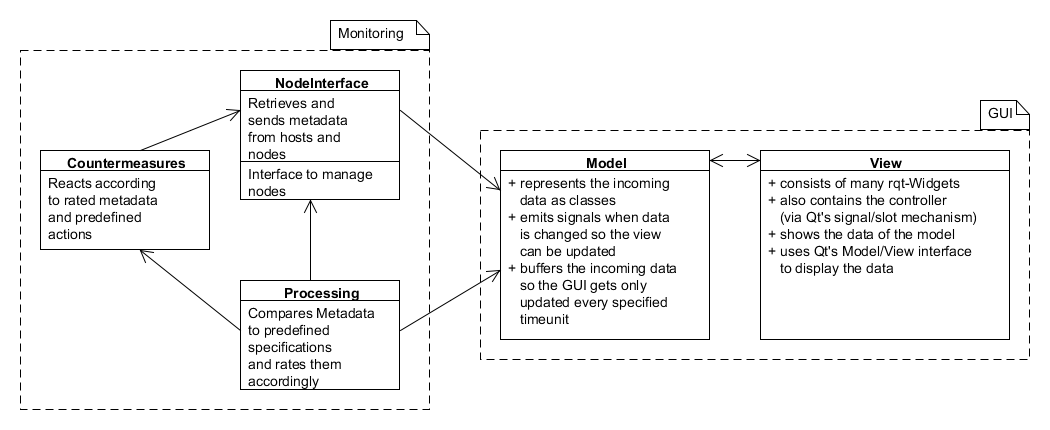
\includegraphics[width=\linewidth]{./bilder/architektur.png}
\caption{This Figure shows the Architecture divided into two major parts, the right depicting the UI and the left depicting the monitoring aspect. The GUI is designed using the Qt MVC architecture. The monitoring aspect is divided into three parts : NodeInterface, Countermeasure and Processing.}
\label{fig:architecture}
\end{figure}

Figure ~\ref{fig:architecture} shows the general architecture of our software. It is divided into two parts, one for the graphical user interface and one for the monitoring aspect.
The right part depicts the GUI. It is designed using the Qt MVC architecture, consisting of only two elements because Qt takes care of the controller: model and view. It will handle user-interaction.
The left part depicts the monitoring aspect. It consists of three elements : NodeInterface, Countermeasure and Processing. It will take care of collecting metadata, processing it and taking appropriate action in case of an error.

\subsection{Monitoring}

\begin{description}
	\item[NodeInterface] \mbox{}
		\begin{itemize}
			\item Retrieves and sends metadata from hosts and nodes.
			\item Interface to manage nodes.
		\end{itemize}
	\item[Processing] \mbox{} 
	Compares Metadata to predefined specifications and
	rates the accordingly.
	\item[Countermeasures] \mbox{} 
	Reacts according to rated metadata and
	predefined actions.
\end{description}

\subsection{GUI}

\begin{description}
	\item[Model] \mbox{}	
		\begin{itemize}
		\item Represents the incoming data as classes.
		\item Emits signals when data is changed so the view can be updated.
		\item Buffers the incoming data so the GUI gets only updated every specified timeunit.
		\end{itemize}
	\item[View] \mbox{}
		\begin{itemize}
		\item Consists of many rqt-Widgets.
		\item Also contains the controller (via Qt's signal/slot mechanism).
		\item Shows the data of the model.
		\item Uses Qt's Model/View interface to display the data.
		\item Also uses pyqtgraph to dynamically plot the incoming data.
		\end{itemize}
\end{description}